\chapter{Emotion Classification Approaches}

In this chapter we will proprose some of the first experiments we made for this
project. Specifically, we will show how we tried to build some first models, solely 
based on the MoodyLyrics dataset, with no particular preprocessing nor feature
engineering techniques, just by using the tools we already mentioned.

After that we will provide a formal validation of one of the tools we used, in
order to make sure that what we have at our disposal is good for our task.

%%%%%%%%%%%%%%%%%%%%%%%%%%%%%%%%%%%%%%%%%%%%%%%%%
%%%%%%%%%%%%%%%%%%%%%%%%%%%%%%%%%%%%%%%%%%%%%%%%%
%%%%%%%%%%%%%%%%%%%%%%%%%%%%%%%%%%%%%%%%%%%%%%%%%
%%%%%%%%%%%%%%%%%%%%%%%%%%%%%%%%%%%%%%%%%%%%%%%%%
%%%%%%%%%%%%%%%%%%%%%%%%%%%%%%%%%%%%%%%%%%%%%%%%%
\section{Initial Classification}

The first approaches to classify emotions we tried, were entirely based on converting
MoodyLyrics entries into features. Specifically, since MoodyLyrics simply provide the
artist and the title of its songs, we fristly downloaded the lyrics and then we built
word embedding vectors for them by using SpaCy's built-in methods, based on word2vec.
Those vectors we worked on are made of 300 dimensions.

No particular preprocessing was applied on lyrics before generating the word embedding
vectors apart from stopword removals, because we did not believe that they could bring
any useful additional information.

\begin{figure}
  \centering
  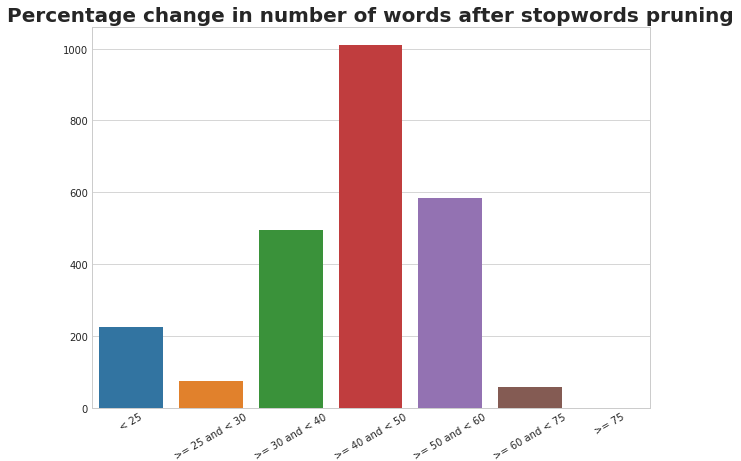
\includegraphics[width=0.9\textwidth]{./chapters/chapter4/images/percentage-change.png}
  \caption{Number of songs and percentage of word in which they changed after stop word removal}
  \label{fig:ml-percentage-change}
\end{figure}

At first we were scared of the fact that most of the words in some lyrics may have been
stop words, ending up in reducing lyrics text by too many words. Anyway, as we can see 
from figure \ref{fig:ml-percentage-change}, less than 650 songs reduced their size by 
more than 50\% while the majority of them has very small percentage decrease. Therefore
we concluded that it could be worth trying to classify our lyrics by applying this mentioned
preprocessing technique.

\begin{figure}
  \centering
  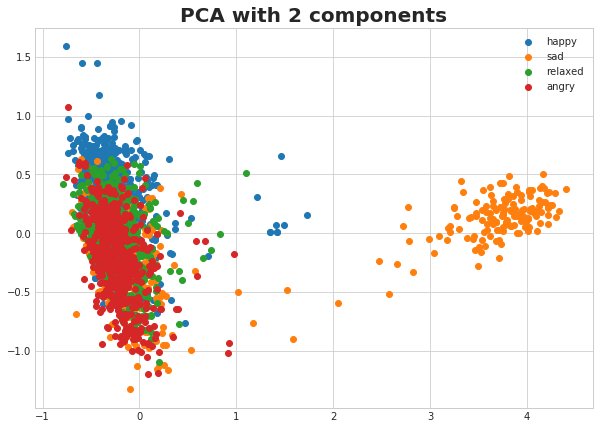
\includegraphics[width=0.9\textwidth]{./chapters/chapter4/images/ml-pca.png}
  \caption{Principal Component Analys on MoodyLyrics data with 2 dimensions as output}
  \label{fig:ml-pca}
\end{figure}

MoodyLyrics songs were annotated according to the arousal and valence dimension of their lyric,
as explained above. Therefore we tought that, if we could be able to project the resulting
word embedding vector of each lyric in a bi-dimensional space, we could have been able to 
clearly see how they are separated.

In order to visualize the mentioned idea, we apply Principal Component Analysis (PCA) on
MoodyLyrics songs and plotted the resulting points in 2-dimensional space, as can be seen in 
figure \ref{fig:ml-pca}. However the resulting figure is not exactly what we were expecting.

Indeed, because of the explained MoodyLyrics annotation schema, we were expecting to see 4
clearly separated group of points. Instead, what we can see is that sad songs are clearly 
separated from the others while the songs belonging to the classes happy, angry and relaxed
are quite overlapped and can be easily confused between them.

Despite the fact that this result seemed weird, after listening to several songs and trying to
manually classify them according to their lyrics, we came to the conclusion that it is very
easy for a human to confuse happy, angry and relaxed song. Therefore, if we keep in mind that
MoodyLyrics was manually annotated, we can explain the anomaly in our plot as a consequence
of human error during the annotation process.

\begin{table}[]
\centering
\begin{tabular}{@{}lll@{}}
\toprule
\textbf{Classifier} & \textbf{Accuracy})   \\ \midrule
k-Nearest Neighbour & 82\%  \\
Support Vector Machine & 90\%  \\
Gradient Boost & 86\%  \\
Neural Network & 90.06\%  \\
\end{tabular}
\caption{Accuracy results for different classifiers on MoodyLyrics}
\label{table:ml-simple-results}
\end{table}

After this preliminary data analysis, we moved on producing models to actually classify our dataset.
The result of these process are visible in table \ref{table:ml-simple-results} where the reported
accuracy values were obtain after a 5-fold cross validation.

As we can see, the best results were certainly achieved by a Neural Network whose architecture was
as follows: one input layer with 60 neurons and sigmoid activation function, one hidden layer with
60 neurons and sigmoid activation function, one output layer with 4 neurons and softmax activation
function.

\begin{table}[]
\centering
\begin{tabular}{@{}lll@{}}
\toprule
\textbf{Classifier} & \textbf{Accuracy})   \\ \midrule
k-Nearest Neighbour & 82\%  \\
Support Vector Machine & 90\%  \\
Gradient Boost & 86\%  \\
Neural Network & 90.06\%  \\
\end{tabular}
\caption{Accuracy results for different classifiers on MoodyLyrics, using just the title's word embedding vector}
\label{table:ml-simple-results-title}
\end{table}

Anyway for certain songs we noticed that the expressed emotion could be easily guessed from its title. Therefore
we tried to build also songs titles word embedding vectors and classified them. The results of this operation are 
visible in table \ref{table:ml-simple-results-title}. Again, those results were obtained after a 5-fold cross-validation. 

\begin{table}[]
\centering
\begin{tabular}{@{}lll@{}}
\toprule
\textbf{Classifier} & \textbf{Accuracy})   \\ \midrule
Support Vector Machine & 62\%  \\
Neural Network & 31.22\%  \\
\end{tabular}
\caption{Accuracy results for different classifiers on MoodyLyrics, using both the lyric's and the title's word embedding vectors}
\label{table:ml-simple-results-both}
\end{table}

Moreover, performances obtained while building classifier based on the songs title's word embedding vector only
did not improve with respect to the previous case even if their decrease was not that high. Therefore we decided
that, probably, we could have given a try at classifying based on both the title's and the lyric's vector for each
song. The results of this process are shown in table \ref{table:ml-simple-results-both}.

For this case we did not try to learn the same number of classifiers as above simply because we noticed a huge decrease
in performances for those models in which we used to obtain the best results. Anyway, this approach was clearly proven to be
the worst so far.

In conclusion, the best performances were those obtained by learning our model solely on the lyrics word embedding vectors.
Those results are also quite encouraging and made us think that, with some more advanced feature engineering techniques,
we may be able to achieve even better results.

%%%%%%%%%%%%%%%%%%%%%%%%%%%%%%%%%%%%%%%%%%%%%%%%%
%%%%%%%%%%%%%%%%%%%%%%%%%%%%%%%%%%%%%%%%%%%%%%%%%
%%%%%%%%%%%%%%%%%%%%%%%%%%%%%%%%%%%%%%%%%%%%%%%%%
%%%%%%%%%%%%%%%%%%%%%%%%%%%%%%%%%%%%%%%%%%%%%%%%%
%%%%%%%%%%%%%%%%%%%%%%%%%%%%%%%%%%%%%%%%%%%%%%%%%
\section{POS Tagger Validity Check} 

Before digging into more complex types of analysis, we took the time to check if
the tools we were using could be really good for our purpose. 

Specifically, we had some doubts on the Part-Of-Speech (POS) tagger. Indeed, those kind of systems are generarly 
trained on texts coming from sources whose type of language is very different from those
we would expect to find in lyrics. In fact, the SpaCy's POS tagger implemented in the language
model we are using is trained on OntoNotes 5\cite{ontonotes5} and on Common Crawl\cite{common-crawl},
which are both made of pieces of text taken from news, conversational telephone speech, weblogs, 
usenet newsgroups, broadcast and talk shows. Obviously, this type of natural language texts are 
much different from a lyric and we just wanted to make sure that we were using a appropriate tool.

Before going into the details of what we did, we must state that SpaCy's POS tagger provides two tags per words, which
will both be considered in our analysis. Those two type of tags are:

\begin{itemize}
\item \textbf{POS}: coarse-grained part-of-speech e.g. VERB
\item \textbf{TAG}: fine-grained part-of-speech e.g. PAST\_TENSE
\end{itemize}

In order to obtain reliable insights of the functionalities of our POS tagger we considered three songs:
one with a common language and very few slang words, one filled with slangs and another one with some
vulgar words.

The first song we considered was "Polly" from Nirvana.

As a first approach we tried to tag the words considering one line of the lyric at the time. Here is an example of
what we obtained:

\begin{lstlisting}
Polly wants a cracker
PROPN VERB DET NOUN 

Polly = PROPN NNP -> noun, proper singular
wants = VERB VBZ -> verb, 3rd person singular present
a = DET DT -> determiner
cracker = NOUN NN -> noun, singular or mass
\end{lstlisting}

As a first attempt, our POS tagger completelly succedeed in recognizing the phrase the 
exact way we were expecting. In fact, the absence of weird words e.g. slangs made the
task much easier.

Because of the almost complete absence of punctuation marks in our lyric, we expected
the POS tagger to fail while analyzing the entire song as whole. Instead, we were quite
surprised to see that SpaCy's POS tagger does one desirable thing for our goal:
it treats each line as a standalone sentence, evern though they are not specifically separed by
a stopping mark. Therefore, the same positive behaviour we observed on the first line
was totally replicated on the other lines, giving us the exact tagging we were
expecting by visually inspecting our song's lyrics.

We omitted the entire tagging process output for brevity reasons.

Our first experiment served to the purpose of arriving to a conclusion: SpaCy's POS tagger
is a good tool for lyrics. However it did not solve our doubts about its ability of recognizing
"weirder" words such as slang words or abbreviations. For this reason, we moved on 
analysing the lyrics of "Kiss You Back" from Underground Kiss.

The first interesting thing we noticed was that the POS tagger properly recognized abbreviations such as "'ll'".
Moreover, another important feature we noticed was clearly visible while tagging this line: "Yeah, we chocolate cross-over".
Indeed, here the word "chocolate" is used as a verb (even though chocolate is clearly not defined as a verb in 
the dictionary) and the POS tagger was able to recognize this exception. 
This is quite important because, in songs, those situations happen very often.

Other additional things we noticed while analyzing this song came our of the tagging output of the following line:

\begin{lstlisting}
Jus't havin' fun with it, man, know what I'm sayin'?
NOUN VERB NOUN ADP PRON PUNCT INTJ PUNCT VERB NOUN PRON VERB VERB PUNCT PUNCT 

Jus't = NOUN NNS -> noun, plural
havin' = VERB VBG -> verb, gerund or present participle
fun = NOUN NN -> noun, singular or mass
with = ADP IN -> conjunction, subordinating or preposition
it = PRON PRP -> pronoun, personal
, = PUNCT , -> punctuation mark, comma
man = INTJ UH -> interjection
, = PUNCT , -> punctuation mark, comma
know = VERB VB -> verb, base form
what = NOUN WP -> wh-pronoun, personal
I = PRON PRP -> pronoun, personal
'm = VERB VBP -> verb, non-3rd person singular present
sayin = VERB VBG -> verb, gerund or present participle
' = PUNCT '' -> closing quotation mark
? = PUNCT . -> punctuation mark, sentence closer
\end{lstlisting}

One very interesting result we can notice comes from the following two lines:
\begin{lstlisting}
havin' = VERB VBG -> verb, gerund or present participle and
ayin = VERB VBG -> verb, gerund or present participle
\end{lstlisting}

In fact it looks like our POS tagger is able to recognize verbs in their correct tense
even if they are abbreviated in an unconventional way.

One thing which really impressed us, was the word "man" being recognized to be an interjection from time to time. 
"An interjection is a part of speech that shows the emotion or feeling of the author. These words or phrases can 
stand alone or be placed before or after a sentence. Many times an interjection is followed 
by a punctuation mark, often an exclamation point"\footnote{\url{http://examples.yourdictionary.com/examples-of-interjections.html}}. 
This description perfectly fits with the usage of the word "man" in their contextes when it was recognized to be an interjection. 

Those kind of things are not trivial to detect and this ability of our POS tagger convinced us even more
of its impressive skills.

The last thing we were left to analyze at this point was a vulgar song. For this purpose we considered 
"The Ballad Of Chasey Lain", from Bloodhound Gang. 

In this case we have no special remarks to report. We can just say that everything was tagged and
recognized in the exact way we expected.

We did not report entire lyrics nor the full POS tagger output for the interest of brevity. However, those
analysis are available on the public GitHub repository for this project\footnote{\url{https://github.com/sgiammy/emotion-patterns-in-music-playlists/blob/master/Notebook/3\_POS\_tagger\_verification.ipynb}}.